\documentclass{article}
\usepackage{geometry,tikz,amsmath}
\usetikzlibrary{backgrounds}
\geometry{%
paperwidth=13cm,
paperheight=11.5cm,
top=1pt,
bottom=0pt,
left=1pt,
right=0pt
}
\setlength{\parindent}{0pt}
\begin{document}
\pagestyle{empty}
\centering
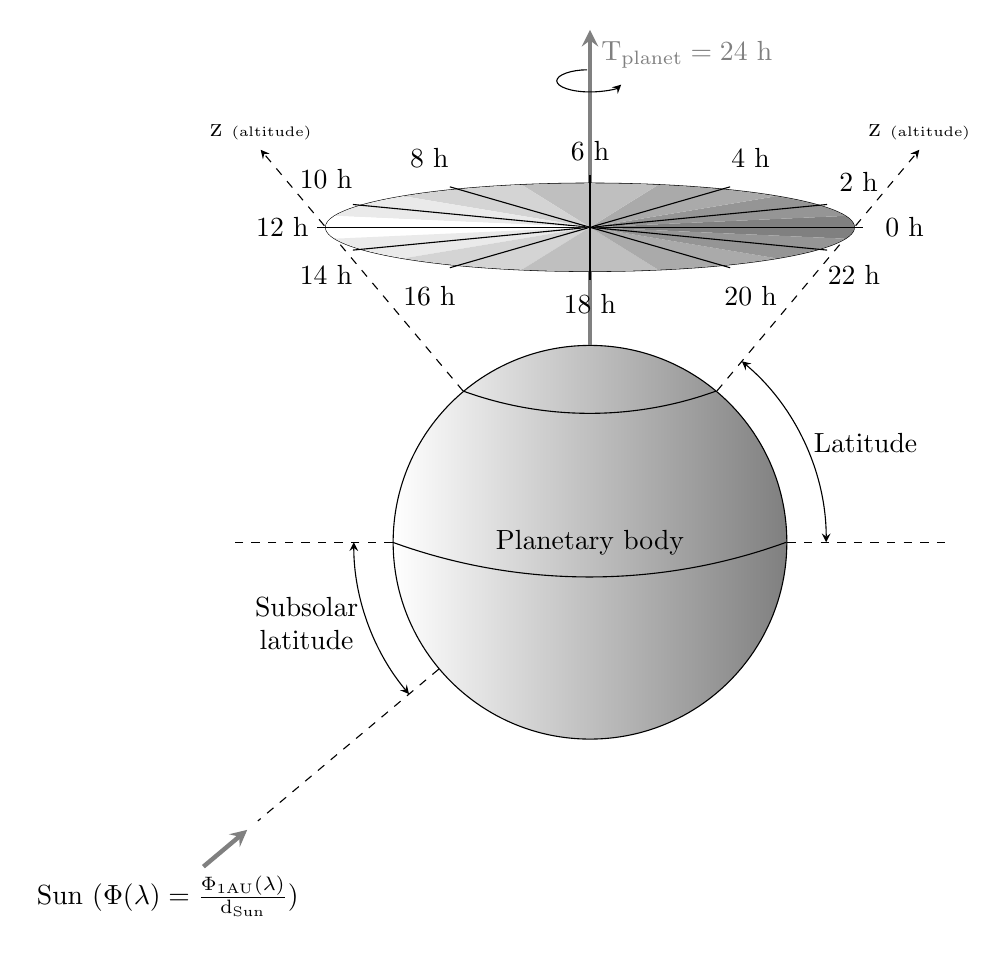
\begin{tikzpicture}[tight background]
%Titan
\node[circle,right color=gray,left color=white,draw,minimum size=5cm] (Titan) at (0,0) {Planetary body};
\pgfmathparse{2.5/sin(20)}\let\dia\pgfmathresult
\draw (Titan.west) arc(-110:-70:\dia);
\draw[dashed] (Titan.west) -- ++(-2,0) 
              (Titan.east) -- ++(2,0);
%altitude
\pgfmathparse{130}\let\alt\pgfmathresult
\pgfmathparse{180-\alt}\let\altc\pgfmathresult
\pgfmathparse{2.5*sin(\alt-90)/sin(20)}\let\dia\pgfmathresult
\draw (Titan.\alt) arc(-110:-70:\dia);
\draw[-stealth,dashed] (Titan.\alt) --++(\alt:4)node[above]{z \tiny(altitude)};
\draw[-stealth,dashed] (Titan.\altc) --++(\altc:4)node[above]{z \tiny(altitude)};
\draw[stealth-stealth] (0:3cm) arc(0:\altc:3cm);
\node[right] at (\altc/2:3cm) {Latitude};
%Sun
\pgfmathparse{220}\let\sun\pgfmathresult
\node (sun) at (\sun:7cm) {Sun ($\Phi(\lambda) = \frac{\Phi_{\text{1AU}}(\lambda)}{\text{d}_{\text{Sun}}}$)};
\draw[dashed] (Titan.\sun) -- ++(\sun:3cm)coordinate(entry);
\draw[-stealth,shorten >=5pt,ultra thick,gray] (sun) edge (entry);
\draw[stealth-stealth] (180:3cm) arc(180:\sun:3cm);
\node[left,align=center] at (90+\sun/2:3cm) {Subsolar\\latitude};
%hours
\draw[ultra thick,gray,-stealth] (Titan.north) --++(0,4cm) node[below right]{$\mathrm{T_{planet}}=24$~h};
\draw[-stealth,shorten <=1pt] (90:6cm) arc(90:340:12pt and 4pt);
\pgfmathparse{sin((\alt-\altc)/2)*4/sin(\altc)}\let\xhour\pgfmathresult
\pgfmathparse{\xhour/6}\let\yhour\pgfmathresult
\draw (90:4cm) circle(\xhour cm and \yhour cm);
\foreach \time in {0,2,...,22}
{
  \pgfmathparse{360/24*\time}\let\ang\pgfmathresult
  \pgfmathparse{360/24*(\time-1)}\let\startarc\pgfmathresult
  \pgfmathparse{360/24*(\time+1)}\let\endarc\pgfmathresult
  \pgfmathparse{200/24*abs(12-\time)}\let\col\pgfmathresult
  \fill[gray!\col] (90:4cm) --++(\startarc:\xhour cm and \yhour cm) arc(\startarc:\endarc:\xhour cm and \yhour cm) -- cycle;
  \draw[shorten >=-3pt] (90:4cm)-- ++(\ang:\xhour cm and \yhour cm)node[pos=1.3,anchor=-\ang]{\time~h}; 
} 
\end{tikzpicture}
\end{document}
